\documentclass[xcolor=dvipsnames,mathserif,9pt]{beamer} %handout
%\usefonttheme{serif}%{structurebold}%{structuresmallcapsserif}%{serif}

%\input{before_document}
\usepackage{graphicx}
\usepackage{amsmath}
\usepackage{amssymb}
\usepackage[font=footnotesize]{caption} % set the captain font size to 8 (i.e. footnotesize)
\usepackage{subfig} % uses subfloats within a single float MUST after the package {caption}!!
\usepackage{natbib}
%\usepackage{cite} % sort the reference in the article by number or alphabatic
\usepackage{color}
\usepackage{algorithm} % options: boxed [section]
\usepackage{algpseudocode} % for algorithm
%\usepackage{enumerate}
\usepackage{enumitem} % directly use itemize, easily specify indent and everything
\setlist[itemize]{leftmargin=*,label=$\bullet$}%leftmargin=*,itemsep=0pt} %topsep=5pt
\setlist[enumerate]{label={\arabic*)}}
\usepackage{hyperref}
\usepackage{wrapfig}
\usepackage{textpos}
\usepackage{bibentry} % for publication list
\makeatletter\let\saved@bibitem\@bibitem\makeatother % make hyperref and bibentry compatible!!!
\nobibliography*
\usepackage{fancybox}% shadow for image
%\usepackage{empheq} % emphasize equations
\usepackage{bm}
\usepackage{arydshln} % for dashline in table or matrix
\linespread{1.3}
\usepackage{multimedia}

\usepackage{setspace} \setstretch{1.2}

\usepackage{framed}
\colorlet{shadecolor}{black!5}
% for box, page breakable, very good!!
\usepackage[framemethod=TikZ]{mdframed}%
\mdfdefinestyle{myFrame}{%
    linecolor=gray!15!white,%gray
    outerlinewidth=0.1pt,
    roundcorner=3pt,
    skipabove=15pt, % the space before the entire box
    skipbelow=15pt, % the space after the entire box. Please see the figure 2 in the manual, very clear!
    innertopmargin=10pt,%\baselineskip,
    innerbottommargin=10pt,%\baselineskip,
    %innerrightmargin=10pt,
    %innerleftmargin=10pt,
    splittopskip=\baselineskip,
    splitbottomskip=\baselineskip,
    backgroundcolor=gray!10!white,
    frametitlerule=true,
    frametitlebackgroundcolor=gray!20!white,
    frametitleaboveskip=5pt,
    frametitlebelowskip=5pt,
}
\mdfdefinestyle{myAlgo}{%
    linecolor=gray!100!white,%gray
    outerlinewidth=0.1pt,
    roundcorner=3pt,
    skipabove=15pt, % the space before the entire box
    skipbelow=15pt, % the space after the entire box. Please see the figure 2 in the manual, very clear!
    innertopmargin=10pt,%\baselineskip,
    innerbottommargin=10pt,%\baselineskip,
    %innerrightmargin=10pt,
    %innerleftmargin=10pt,
    splittopskip=\baselineskip,
    splitbottomskip=\baselineskip,
    backgroundcolor=gray!0!white,
    frametitlerule=true,
    frametitlebackgroundcolor=gray!20!white,
    frametitleaboveskip=5pt,
    frametitlebelowskip=5pt,
}


\usepackage{tikz}
\usetikzlibrary{calc} % for calculation functions in Tikz let, in commands in Tikz
\usetikzlibrary{shapes} % for block diagram
\usetikzlibrary{chains}
\usetikzlibrary{fit}
\usetikzlibrary{arrows}
\usetikzlibrary{decorations.text} % text along path

\newcommand{\blue}[1]{\textcolor{blue}{#1}}
\definecolor{myred}{RGB}{200,0,0}
\newcommand{\red}[1]{\textcolor{myred}{#1}} %magenta purple
\newcommand{\I}{\mathcal{I}}
\newcommand{\tr}{\mathrm{tr}}
\newcommand{\Null}{\mathrm{Null}}
\newcommand{\Range}{\mathrm{Range}}
\newcommand{\one}{\mathbf{1}}
\newcommand{\rank}{\mathrm{rank}}
\newcommand{\myspan}{\mathrm{span}}
\newcommand{\mydiag}{\mathrm{diag}}
\newcommand{\D}{\mathrm{d}}
\renewcommand{\d}{\mathrm{d}}
\newcommand{\blkdiag}{\mathrm{blkdiag}}
\newcommand{\sgn}{\mathrm{sgn}}
\newcommand{\T}{\mathrm{T}}
\newcommand{\myqed}{\hfill$\blacksquare$}
\newcommand{\ep}{\varepsilon}
\newcommand{\sig}{\mathrm{sig}_a}
%\newcommand{\sigep_}[1]{\sig(\ep_{#1})}
\newcommand{\R}{\mathbb{R}}
\newcommand{\A}{\mathcal{A}}
\newcommand{\G}{\mathcal{G}}
\newcommand{\E}{\mathbb{E}}
\newcommand{\X}{\mathcal{X}}
\newcommand{\V}{\mathcal{V}}
\newcommand{\N}{\mathcal{N}}
\newcommand{\M}{\mathcal{M}}
\renewcommand{\H}{\mathcal{H}}
\renewcommand{\L}{\mathcal{B}}
\renewcommand{\S}{\mathcal{S}}
\newcommand{\xe}{x_{\text{e}}}
%\newcommand{\Null}[1]{\mathrm{Null}\left(#1\right)}
\newcommand{\sk}[1]{\left[#1\right]_\times} % skew symmetric operator
\newcommand{\dia}[1]{\mathrm{diag}\left(#1\right)} % block diagnal matrix
%\renewcommand{\span}[1]{\mathrm{span}\left\{#1\right\}} % ERROR when redefine \span
\newcommand{\Var}{\mathrm{Var}}
\newcommand{\var}{\mathrm{var}}


\graphicspath{{figures/}}

% for tikz, theorem, lemma ... environments have already been declared. You don't need to declare, or you need to use other names than theorem or lemma, such as my_theorem.
%\newtheorem{my_theorem}{Theorem}
%\newtheorem{my_lemma}{Lemma}
\newtheorem{assumption}{Assumption} % necessary for beamer
%\newtheorem{my_remark}{Remark}
\newtheorem{proposition}{Proposition} % necessary for beamer
%\newtheorem{my_corollary}{Corollary}
%\newtheorem{my_example}{Example}
%\newtheorem{my_definition}{Definition}
%\newtheorem{my_problem}{Problem}

%##################################################
\newcommand{\pagetitle}[1]{\textbf{\textcolor{BlueViolet}{$\circ$ #1}}} %!!!
\newcommand{\pagehighlight}[1]{\textbf{\textcolor{Brown}{#1}}} %!!!
\newcommand{\mypause}{\pause} % this is useful for slide show. if you don't want pause any more, just set it as blank
%\newcommand{\mybullet}{\textcolor{BlueViolet}{$\blacksquare$} }%{$\rhd$ }
%\newcommand{\myhighsign}{$\star$ }% the sign to highlight a sentence

%##################################################
% To highlight equation. Example: \begin{align*} \boxed{xxx} \end{align*}
% does not support multiline equations
% put color to \boxed math command
\newcommand*{\boxcolor}{gray}
\makeatletter
\renewcommand{\boxed}[1]{\textcolor{\boxcolor}{%
%\tikz[baseline={([yshift=-1ex]current bounding box.center)}] \node [rectangle, minimum width=1ex,rounded corners,draw] {\normalcolor\m@th$\displaystyle#1$};}}
\tikz[baseline={([yshift=-1ex]current bounding box.center)}] \node [rectangle, minimum width=2ex,rounded corners,draw] {\normalcolor\m@th$\displaystyle#1$};}}
\makeatother

%##################################################
% set my own theme
\def\structureHeight{9mm}
\usetheme[height=\structureHeight]{Rochester}
\usecolortheme[RGB={0,0,128}]{structure}
\setbeamertemplate{items}[circle]%rectangle, triangle,circle
\setbeamertemplate{blocks}[rounded][shadow=true]
\setbeamertemplate{navigation symbols}{}
%\addtobeamertemplate{frametitle}{} % specify the logo
%{
%    \begin{textblock*}{100mm}(.87\textwidth,-\structureHeight)
%        \includegraphics[height=6.6mm,width=3cm,keepaspectratio]{../common_figures_private/westlake_logo.png} % add logo
%    \end{textblock*}
%}
\addtobeamertemplate{frametitle}{\vskip4pt}{} % specify
%\setbeamerfont{frametitle}{size=\large}
\definecolor{mylightgray}{RGB}{240 240 240}
\definecolor{mykhaki}{RGB}{240 230 140}% khaki color
\definecolor{mylightYellow}{RGB}{255,255,224} % light yellow
%\setbeamercolor{beamercolor1}{bg=mylightgray, fg=black}
%\setbeamercolor{beamercolor2}{bg=mylightYellow,fg=black}%{bg=yellow!90!white, fg=black}
% background and foreground color
\setbeamercolor{background canvas}{bg=black!0!white} % background color of every slide! My previous value was black!10!white for my lecture videos!
\setbeamercolor{normal text}{bg=black!10!white} % background color for e.g. theorem environment. When canvas is 10, here it can be 20; the bg for normal text changes the color of hidden text when you use overlay

\setbeamercolor{block title}{bg=mykhaki,fg=black}
\defbeamertemplate{footline}{zsy_frameNumber}
{%
  \hspace{5pt}  \emph{Shiyu Zhao}
  \hspace*{\fill}%
  \usebeamercolor[fg]{page number in head/foot}%
  \insertframenumber\,/\,\inserttotalframenumber \vspace{0pt} \hspace{5pt}
  \vskip5pt
}
\setbeamertemplate{footline}[zsy_frameNumber]
%##################################################
\setbeamercovered{transparent=0} % a good value for transparent text is 20
% when using the overlay commands like \onslide or \uncover, the text will NOT be invisible, instead it will be like transparent
%\pause will also have the transparent effect: command \pause is easy to use: to make it invisible, change the value to zero.



\usepackage{multimedia}

\newcommand{\hl}{$\triangleright$ }
%\newcommand{\blue}[1]{\textcolor{blue}{#1}}
%\newcommand{\red}[1]{\textcolor{red}{#1}}



\begin{document}

%%%%%%%%%%%%%%%%%%%%%%%%%%%%%%%%%%%%%%%%%%%%%%%%%%%%%%%%%%%%%%%%%%%%%%%%%%%%%%%%%
% define the author, date etc. information
%\subtitle{Mathematical and Biological Foundation for Reinforcement Learning}
\title{Lecture 2: State Value and Bellman Equation}

\author{Shiyu Zhao
\newline
\newline {\small Department of Artificial Intelligence}
\newline {\small Westlake University}
}
%\logo{\includegraphics[width=1cm,height=1cm,keepaspectratio]{NUSLogo.png}~}
%\date{\today}
\date{}
\subject{}


%%%%%%%%%%%%%%%%%%%%%%%%%%%%%%%%%%%%%%%%%%%%%%%%%%%%%%%%%%%%%%%%%%%%%%%%%%%%%%%%%

{
\setbeamertemplate{footline}{} % remove the frame number of the title page
\begin{frame}
    %\frametitle{Lecture: Networked Dynamic Systems}
    \addtocounter{framenumber}{-1} % discounter the title page, otherwise the frame number starts from 2 instead of 1
    \titlepage % this only gives the author etc. information
\end{frame}
}



%------------------------------------------
\begin{frame}
\frametitle{Outline}
\begin{figure}[h]
  \centering
\includegraphics[width=0.8\linewidth]{Figure_chapterRelationship.pdf}
\end{figure}
\end{frame}

%\begin{frame}
%\frametitle{Outline}
%
%\begin{itemize}
%\item Model-based algorithms:
%\begin{itemize}
%\item Must know the math model of the environment: $p(s'|s,a)$ and $p(r|s,a)$
%\item For example, value iteration and policy iteration algorithms
%\end{itemize}
%\pause
%\item Model-free algorithms:
%\begin{itemize}
%\item Does not require to know $p(s'|s,a)$ and $p(r|s,a)$
%\item From now on, we will study model-free algorithms!
%\end{itemize}
%\end{itemize}
%
%\end{frame}

\begin{frame}
\frametitle{Outline}
\tableofcontents
\end{frame}
\AtBeginSection[]% put it to the start of each section
{
  \begin{frame}
    \frametitle{Outline}
    \tableofcontents[currentsection]
  \end{frame}
}
%--------------------------------------
\AtBeginSection[]% put it to the start of each section
{
  \begin{frame}
    \frametitle{Outline}
    \tableofcontents[currentsection]
  \end{frame}
}
\section{Motivating example}

%----------------------------------
\begin{frame}
\frametitle{Motivating example: Monte Carlo estimation}

\hl How can we estimate something \textbf{without models}?
\begin{itemize}
\item The simplest idea: \emph{Monte Carlo estimation}.
\end{itemize}

\pause
\vspace{10pt}
\hl \textbf{Example: Flip a coin}

\vspace{10pt}
The result (either head or tail) is denoted as a random variable $X$
\begin{itemize}
\item if the result is head, then $X=+1$
\item if the result is tail, then $X=-1$
\end{itemize}

\vspace{10pt}
The \emph{aim} is to compute $\E[X]$.

\end{frame}
%----------------------------------
\begin{frame}
\frametitle{Motivating example: Monte Carlo estimation}

\hl \textbf{Method 1: with model}
\begin{itemize}
\item Suppose the probabilistic model is known as
$$p(X=1)=0.5, \quad p(X=-1)=0.5$$
Then by definition
$$\E[X]=\sum_x xp(x)=1\times 0.5+(-1)\times 0.5=0$$
\pause
\item \textbf{Problem: it may be impossible to know the precise distribution!}
\end{itemize}
\end{frame}
%---------------------
\begin{frame}
\frametitle{Motivating example: Monte Carlo estimation}

\hl \textbf{Method 2: without model or called model-free}

\begin{itemize}
\item \emph{Idea:} Flip the coin many times, and then calculate the average of the outcomes.

\pause
\item Suppose we get a sample sequence: $\{{x}_1,{x}_2,\dots,{x}_N\}$.

Then, the mean can be approximated as
$$\E[X]\approx\bar{x}=\frac{1}{N}\sum_{j=1}^N {x}_j.$$

This is the idea of Monte Carlo estimation!
\end{itemize}
\end{frame}
%---------------------
\begin{frame}
\frametitle{Motivating example: Monte Carlo estimation}

\hl \textbf{Question:} Is the Monte Carlo estimation accurate?

\begin{itemize}
\item When $N$ is \blue{small}, the approximation is \blue{inaccurate}.
\item When $N$ is \blue{large}, the approximation is \blue{more accurate}.
\end{itemize}
\visible<2->{
\begin{figure}[h!]
\centering
  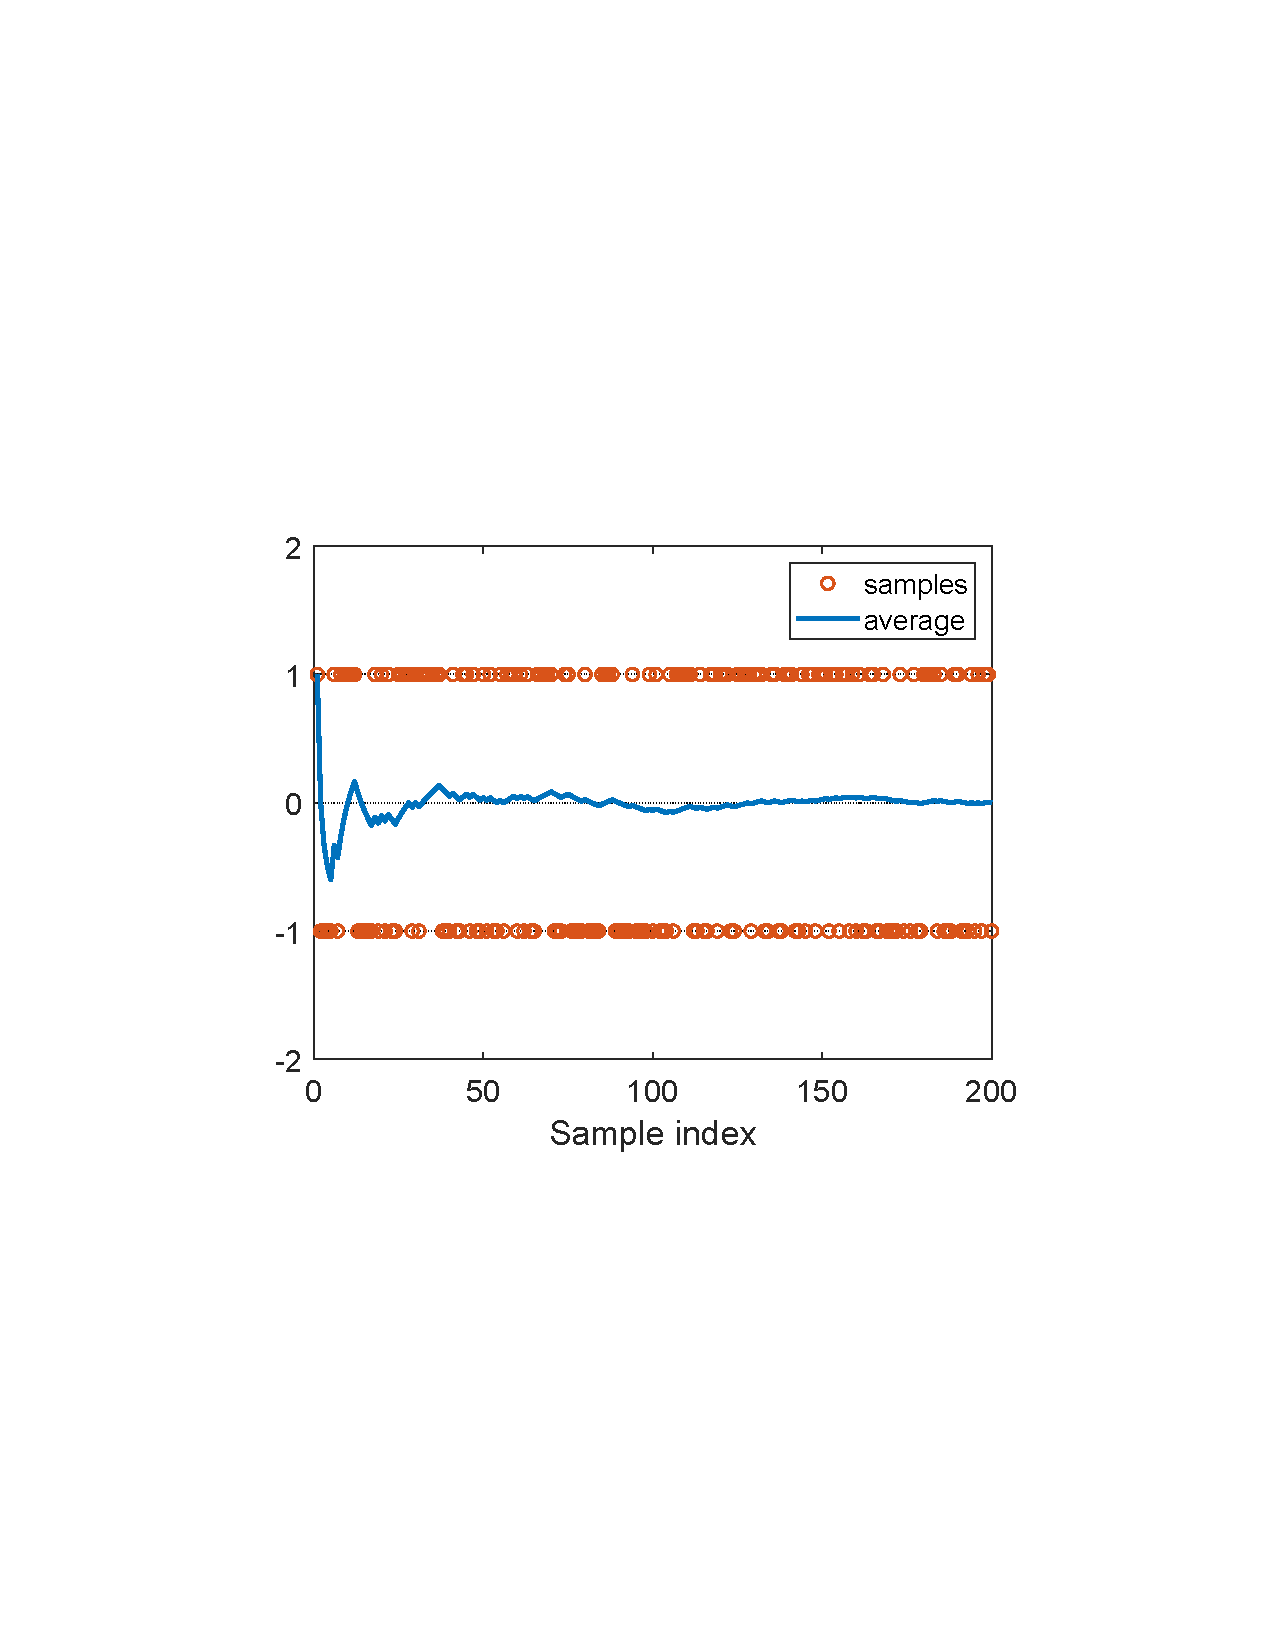
\includegraphics[width=0.6\linewidth]{fig_demoLawLargeNum}
\end{figure}}
\end{frame}
%---------------------
\begin{frame}
\frametitle{Motivating example: Monte Carlo estimation}

\begin{theorem}[Law of Large Numbers]
For a random variable $X$, suppose $\{{x}_j\}_{j=1}^N$ are some iid samples. Let $\bar{x}=\frac{1}{N}\sum_{j=1}^N {x}_j$ be the average of the samples. Then,
\begin{align*}
\E[\bar{x}]&=\E[X],\\
\Var[\bar{x}]&=\frac{1}{N}\Var[X].
\end{align*}
As a result, $\bar{x}$ is an unbiased estimate of $\E[X]$ and its variance decreases to zero as $N$ increases to infinity.
\end{theorem}

\vspace{10pt}
\hl The samples must be \blue{iid (independent and identically distributed)}

\hl For the proof, see the book.
\end{frame}
%---------------------
\begin{frame}
\frametitle{Motivating example: Monte Carlo estimation}
\hl Summary:

\begin{itemize}
\item Monte Carlo estimation refers to a broad class of techniques that rely on repeated random sampling to solve approximation problems.
\pause
\item Why we care about Monte Carlo estimation? Because it does not require the model!
\pause
\item Why we care about mean estimation? Because state value and action value are defined as expectations of random variables!
\end{itemize}

\end{frame}

%--------------------------------------
\AtBeginSection[]% put it to the start of each section
{
  \begin{frame}
    \frametitle{Outline}
    \tableofcontents[currentsection]
  \end{frame}
}
\section{The simplest MC-based RL algorithm}
%---------------------
\begin{frame}
\frametitle{Convert policy iteration to be model-free}

The key idea is to \blue{convert the \emph{policy iteration} algorithm to be model-free.}

\vspace{10pt}
It is simple to understand if you
\begin{itemize}
\item understand the policy iteration algorithm well, and
\item understand the idea of Monte Carlo mean estimation.
\end{itemize}

\end{frame}
%---------------------
\begin{frame}
\frametitle{Convert policy iteration to be model-free}

Policy iteration has two steps in each iteration:
\begin{align*}
\left\{
                                                               \begin{array}{l}
                                                                 \text{\textbf{Policy evaluation:} } v_{\pi_k}=r_{\pi_k}+\gamma  P_{\pi_k} v_{\pi_k} \\
                                                                 \text{\textbf{Policy improvement:} }\pi_{k+1}=\arg\max_{\pi} (r_\pi +\gamma  P_\pi v_{\pi_k})\\
                                                               \end{array}
                                                             \right.
\end{align*}
\pause
The elementwise form of the \textbf{policy improvement step} is:
{\small
\begin{align*}
\textcolor{blue}{\pi_{k+1}(s)}
&=\arg\max_\pi \sum_{a}\pi(a|s)\left[\sum_{r}p(r|s,a)r + \gamma\sum_{s'}p(s'|s,a){v_{\pi_k}(s')}\right]\\
&\textcolor{blue}{=\arg\max_\pi \sum_{a}\pi(a|s)\textcolor{red}{q_{\pi_k}(s,a)}},\quad s\in\mathcal{S}
\end{align*}
}
\pause
The key is to calculate $\textcolor{red}{q_{\pi_k}(s,a)}$!

\end{frame}
%---------------------
\begin{frame}
\frametitle{Convert policy iteration to be model-free}

Two expressions of action value:
\begin{itemize}
\item \textbf{Expression 1 requires the model:}
\begin{align*}
q_{\pi_k}(s,a)=\sum_{r}p(r|s,a)r + \gamma\sum_{s'}p(s'|s,a)v_{\pi_k}(s')
\end{align*}
\pause
\item  \textbf{Expression 2 does not require the model:}
\begin{align*}
q_{\pi_k}(s,a)
&=\E[G_t|S_t=s,A_t=a]
%&=\E[R_{t+1}+\gamma R_{t+2}+\gamma^2 R_{t+3}+\dots|S_t=s,A_t=a]
\end{align*}
\end{itemize}
\pause
\vspace{10pt}
\blue{Idea to achieve model-free RL:} We can use expression 2 to obtain $q_{\pi_k}(s,a)$ based on \emph{data (samples or experiences)}!

\end{frame}
%---------------------
\begin{frame}
\frametitle{Convert policy iteration to be model-free}

How to obtain $q_{\pi_k}(s,a)$ based on data?
\begin{itemize}
\item Starting from $(s,a)$, following policy $\pi_k$, generate an episode.
\pause
\item The return of this episode is $g(s,a)$, which is a sample of $G_t$ in
\begin{align*}
q_{\pi_k}(s,a)
&=\E[G_t|S_t=s,A_t=a]
\end{align*}
\vspace{-15pt}
\pause
\item Suppose we have a set of episodes and hence $\{g^{(j)}(s,a)\}$. Then,
$$q_{\pi_k}(s,a)=\E[G_t|S_t=s,A_t=a]\approx\frac{1}{N}\sum_{i=1}^N g^{(i)}(s,a).$$
\end{itemize}
\pause
\red{Fundamental idea: When model is unavailable, we can use data.}
\end{frame}
%---------------------
\begin{frame}
\frametitle{The MC Basic algorithm}
Given an initial policy $\pi_0$, there are two steps in the $k$th iteration.

\begin{itemize}
\item \textbf{Step 1: policy evaluation.} This step aims to estimate $q_{\pi_k}(s,a)$ for all $(s,a)$. Specifically, for each $(s,a)$, run sufficiently many episodes. The average of their returns, denoted as $q_k(s,a)$, is used to approximate $q_{\pi_k}(s,a)$.
\onslide<2->{
\blue{
\begin{itemize}
\item[-] The first step of the \emph{policy iteration algorithm} calculates $q_{\pi_k}(s,a)$ by firstly solving the state values $v_{\pi_k}$ from the Bellman equation. This requires the model.
\item[-] The first step of the \emph{MC Basic algorithm} is to directly estimate $q_k(s,a)$ from experiences samples. This does not require the model.
\end{itemize}
}}
\item \textbf{Step 2: policy improvement.} This step aims to solve $\pi_{k+1}(s)=\arg\max_\pi \sum_{a}\pi(a|s)q_{k}(s,a)$ for all $s\in\S$. The greedy optimal policy is $\pi_{k+1}(a^*_k|s)=1$ where $a^*_k=\arg\max_a q_{k}(s,a)$.
\onslide<3->{
\blue{
\begin{itemize}
\item[-] This step is exactly the same as the second step of the policy iteration algorithm.
\end{itemize}
}}
\end{itemize}

\end{frame}
\subsection{Algorithm: MC Basic}
%---------------------
\begin{frame}
\frametitle{The MC Basic algorithm}
\hl Description of the algorithm:
{\small%footnotesize
\begin{figure}[t]
\begin{mdframed}[style=myAlgo,nobreak=true,frametitle={Pseudocode: MC Basic algorithm (a model-free variant of policy iteration)}]
{\fontfamily{cmss}\selectfont
\textbf{Initialization:} Initial guess $\pi_0$.

\textbf{Aim:} Search for an optimal policy.

\vspace{5pt}
For the $k$th iteration ($k=0,1,2,\dots$), do

\qquad For every state $s\in\S$, do

\qquad\qquad For every action $a\in\A(s)$, do

\setlength{\leftskip}{6em} \textcolor{blue}{Collect sufficiently many episodes starting from $(s,a)$ following $\pi_k$}

\setlength{\leftskip}{6em} \textcolor{blue}{\emph{Policy evaluation:}}

\setlength{\leftskip}{6em} \textcolor{blue}{$q_{\pi_k}(s,a)\approx q_{k}(s,a)=$ average return of all the episodes starting from $(s,a)$}

\setlength{\leftskip}{4em} \emph{Policy improvement:}

\setlength{\leftskip}{4em} $a^*_k(s)=\arg\max_a q_{k}(s,a)$

\qquad\qquad $\pi_{k+1}(a|s)=1$ if $a=a^*_k$, and $\pi_{k+1}(a|s)=0$ otherwise
}
\end{mdframed}
\end{figure}
}
\end{frame}
%---------------------
\begin{frame}
\frametitle{The MC Basic algorithm}

\begin{itemize}
\item MC Basic is a variant of the policy iteration algorithm.
\pause
\item \blue{The model-free algorithms are built up based on model-based ones.} It is, therefore, necessary to understand model-based algorithms first before studying model-free algorithms.
\pause
\item MC Basic is \blue{useful to reveal the core idea} of MC-based model-free RL, but \red{not practical due to low efficiency}.
\pause
\item Why does MC Basic estimate \blue{action values} instead of \blue{state values}?
That is because state values cannot be used to improve policies directly. When models are not available, we should directly estimate action values.
\pause
\item Since policy iteration is convergent, the \emph{convergence} of MC Basic is also guaranteed to be convergent given sufficient episodes.
\end{itemize}
\end{frame}
%---------------------
\begin{frame}
\frametitle{Illustrative example 1: step by step}

\begin{figure}[h]
  \centering
  \includegraphics[width=0.3\linewidth]{fig_MCDemoExample.pdf}
\end{figure}

Task:
\begin{itemize}
\item An initial policy is shown in the figure.

\item Use MC Basic  to find the optimal policy.

\item $r_{\rm boundary}=-1$, $r_{\rm forbidden}=-1$, $r_{\rm target}=1$, $\gamma=0.9$.

\end{itemize}

\end{frame}
%---------------------
\begin{frame}
\frametitle{Illustrative example 1: step by step}
\begin{figure}[h]
  \centering
  \includegraphics[width=0.25\linewidth]{fig_MCDemoExample.pdf}
\end{figure}

Outline: given the current policy $\pi_k$
\begin{itemize}
\item Step 1 - policy evaluation: calculate $q_{\pi_k}(s,a)$

\textcolor{blue}{How many state-action pairs? 9 states $\times$ 5 actions =45 state-action pairs!}

\item Step 2 - policy improvement: select the greedy action $a^*(s)=\arg\max_{a} q_{\pi_k}(s,a)$
\end{itemize}
\end{frame}
%---------------------
\begin{frame}
\frametitle{Illustrative example 1: step by step}
\begin{figure}[h]
  \centering
  \includegraphics[width=0.25\linewidth]{fig_MCDemoExample.pdf}
\end{figure}
\hl Due to space limitation, we only show $q_{\pi_k}(\textcolor{red}{s_1},a)$

\hl \textbf{Step 1 - policy evaluation:}

\begin{itemize}
\item Since the current policy is \blue{deterministic}, \blue{one episode} would be sufficient to get the action value! Otherwise, if the policy or model is stochastic, many episodes are required!
\end{itemize}

\end{frame}
%---------------------
\begin{frame}
\frametitle{Illustrative example 1: step by step}

\begin{figure}[h]
  \centering
  \includegraphics[width=0.2\linewidth]{fig_MCDemoExample.pdf}
\end{figure}

\begin{itemize}
\item Starting from $(s_1,a_1)$, the episode is
$\textcolor{blue}{s_1\xrightarrow{a_1}}\textcolor{red}{s_1\xrightarrow{a_1}s_1\xrightarrow{a_1}\dots}$.
Hence, the action value is
\vspace{-5pt}
$$q_{\pi_0}(s_1,a_1)=-1+\gamma(-1)+\gamma^2(-1)+\dots$$
\pause
\vspace{-15pt}
\item Starting from $(s_1,a_2)$, the episode is
$\textcolor{blue}{s_1\xrightarrow{a_2}}\textcolor{red}{s_2\xrightarrow{a_3}s_5\xrightarrow{a_3}\dots}$.
Hence, the action value is
\vspace{-5pt}
$$q_{\pi_0}(s_1,a_2)=0+\gamma0+\gamma^20+\gamma^3(1)+\gamma^4(1)+\dots$$
\item Starting from $(s_1,a_3)$, the episode is
$\textcolor{blue}{s_1\xrightarrow{a_3}}\textcolor{red}{s_4\xrightarrow{a_2}s_5\xrightarrow{a_3}\dots}$.
Hence, the action value is
\vspace{-5pt}
$$q_{\pi_0}(s_1,a_3)=0+\gamma0+\gamma^20+\gamma^3(1)+\gamma^4(1)+\dots$$
\end{itemize}

\end{frame}
%---------------------
\begin{frame}
\frametitle{Illustrative example 1: step by step}

\begin{figure}[h]
  \centering
  \includegraphics[width=0.2\linewidth]{fig_MCDemoExample.pdf}
\end{figure}
\begin{itemize}
\item Starting from $(s_1,a_4)$, the episode is
$\textcolor{blue}{s_1\xrightarrow{a_4}}\textcolor{red}{s_1\xrightarrow{a_1}s_1\xrightarrow{a_1}\dots}$.
Hence, the action value is
$$q_{\pi_0}(s_1,a_4)=-1+\gamma(-1)+\gamma^2(-1)+\dots$$
\item Starting from $(s_1,a_5)$, the episode is
$\textcolor{blue}{s_1\xrightarrow{a_5}}\textcolor{red}{s_1\xrightarrow{a_1}s_1\xrightarrow{a_1}\dots}$.
Hence, the action value is
$$q_{\pi_0}(s_1,a_5)=0+\gamma(-1)+\gamma^2(-1)+\dots$$
\end{itemize}
\end{frame}
%---------------------
\begin{frame}
\frametitle{Illustrative example 1: step by step}

\begin{figure}[h]
  \centering
  \includegraphics[width=0.2\linewidth]{fig_MCDemoExample.pdf}
\end{figure}

\hl \textbf{Step 2 - policy improvement:}
\begin{itemize}
\item By observing the action values, we see that
$$q_{\pi_0}(s_1,a_2)=q_{\pi_0}(s_1,a_3)$$
are the \emph{maximum}.
\item As a result, the policy can be improved as
$$\pi_{1}(a_2|s_1)=1 \text{\quad or \quad} \pi_{1}(a_3|s_1)=1$$
In either way, the new policy for $s_1$ becomes optimal.
\end{itemize}
One iteration is sufficient for this simple example!
\end{frame}
%---------------------
\begin{frame}
\frametitle{Illustrative example 1: step by step}

\begin{figure}[h]
  \centering
  \includegraphics[width=0.3\linewidth]{fig_MCDemoExample.pdf}
\end{figure}

Exercise: now update the policy for $s_3$ using MC Basic!

\end{frame}%
%%---------------------
%\begin{frame}
%\frametitle{Illustrative example 2: Episode length}
%
%Let's examine \blue{the impact of episode length:}
%\begin{itemize}
%\item We need sample episodes, but the length of an episode cannot be infinitely long. How long should the episodes be?
%\end{itemize}
%\vspace{10pt}
%\pause
%Example setup:
%\begin{itemize}
%\item 5-by-5 grid world
%\item Reward setting: $r_{\rm boundary}=-1$, $r_{\rm forbidden}=-10$, $r_{\rm target}=1$, $\gamma=0.9$
%\end{itemize}
%
%\end{frame}
%%---------------------
%\begin{frame}
%\frametitle{Illustrative example 2: Episode length}
%
%\hl Use MC Basic to search optimal policies with different episode lengths.
%\vspace{-10pt}
%\captionsetup[subfigure]{labelformat=empty}
%\begin{figure}
%  \centering
%  \subfloat[episode length=1]{
%  \includegraphics[width=0.23\linewidth]{fig_gridStateValue_epL1.pdf}
%  \includegraphics[width=0.23\linewidth]{fig_gridPolicy_epL1.pdf}}
%  \visible<2->{
%  \subfloat[episode length=2]{
%  \includegraphics[width=0.23\linewidth]{fig_gridStateValue_epL2.pdf}
%  \includegraphics[width=0.23\linewidth]{fig_gridPolicy_epL2.pdf}}\\}
%  \vspace{-5pt}
%  \visible<3->{
%  \subfloat[episode length=3]{
%  \includegraphics[width=0.23\linewidth]{fig_gridStateValue_epL3.pdf}
%  \includegraphics[width=0.23\linewidth]{fig_gridPolicy_epL3.pdf}}}
%  \visible<4->{
%  \subfloat[episode length=4]{
%  \includegraphics[width=0.23\linewidth]{fig_gridStateValue_epL4.pdf}
%  \includegraphics[width=0.23\linewidth]{fig_gridPolicy_epL4.pdf}}}
%\end{figure}
%\end{frame}
%%---------------------
%\begin{frame}
%\frametitle{Illustrative example 2: Episode length}
%\vspace{-10pt}
%\captionsetup[subfigure]{labelformat=empty}
%\begin{figure}
%  \centering
%  \subfloat[episode length=14]{
%  \includegraphics[width=0.23\linewidth]{fig_gridStateValue_epL14.pdf}
%  \includegraphics[width=0.23\linewidth]{fig_gridPolicy_epL14.pdf}}
%  \visible<2->{
%  \subfloat[episode length=15]{
%  \includegraphics[width=0.23\linewidth]{fig_gridStateValue_epL15.pdf}
%  \includegraphics[width=0.23\linewidth]{fig_gridPolicy_epL15.pdf}}\\}
%  \visible<3->{
%  \subfloat[episode length=30]{
%  \includegraphics[width=0.23\linewidth]{fig_gridStateValue_epL30.pdf}
%  \includegraphics[width=0.23\linewidth]{fig_gridPolicy_epL30.pdf}}}
%  \visible<4->{
%  \subfloat[episode length=100]{
%  \includegraphics[width=0.23\linewidth]{fig_gridStateValue_epL100.pdf}
%  \includegraphics[width=0.23\linewidth]{fig_gridPolicy_epL100.pdf}}}
%\end{figure}
%\end{frame}
%%---------------------
%\begin{frame}
%\frametitle{Illustrative example 2: Episode length}
%\vspace{-10pt}
%\begin{figure}
%  \centering
%  \includegraphics[width=0.245\linewidth]{fig_gridStateValue_epL4.pdf}
%  \includegraphics[width=0.245\linewidth]{fig_gridPolicy_epL4.pdf}
%\end{figure}
%\vspace{-10pt}
%\hl \textbf{Findings:}
%\begin{itemize}
%\item When the episode length is short, only the states that are close to the target have nonzero state values.
%\item As the episode length increases, the states that are closer to the target have nonzero values earlier than those farther away.
%\pause
%\item The episode length should be sufficiently long.
%\item The episode length does not have to be infinitely long.
%\end{itemize}
%
%\end{frame}

%%---------------------
%\begin{frame}
%\frametitle{Illustrative example 2: Episode length}
%
%%\vspace{-10pt}
%\begin{figure}
%  \centering
%  \includegraphics[width=0.245\linewidth]{fig_gridStateValue_epL4.pdf}
%  \includegraphics[width=0.245\linewidth]{fig_gridPolicy_epL4.pdf}
%\end{figure}
%\vspace{-10pt}
%
%\hl \textbf{Related to sparse reward:}
%
%\begin{itemize}
%\item \emph{Sparse reward:}
%\begin{itemize}
%\item Only if the agent reaches the target state, can a positive reward be obtained.
%\item In other words, no positive rewards can be obtained unless the target is reached.
%\end{itemize}
%%\pause
%%\item \emph{Fundamental reason:} episodes cannot be infinitely long!
%\pause
%\item \emph{Solution:} make reward non-sparse!
%\begin{itemize}
%\item Redesign the reward so that the agent can obtain positive rewards when reaching those states located near the target.
%\end{itemize}
%\end{itemize}
%\end{frame}
%--------------------------------------
\AtBeginSection[]% put it to the start of each section
{
  \begin{frame}
    \frametitle{Outline}
    \tableofcontents[currentsection]
  \end{frame}
}
\section{Use data more efficiently}
%---------------------
\begin{frame}
\frametitle{Use data more efficiently}
The MC Basic algorithm:
\begin{itemize}
\item \textbf{Advantage}: reveal the core idea clearly!
\item \textbf{Disadvantage}: too simple to be practical.
\end{itemize}
However, MC Basic can be extended to be more efficient.
\end{frame}
%---------------------
\begin{frame}
\frametitle{Use data more efficiently}

\hl Consider a grid-world example, following a policy $\pi$, we can get an episode such as
$$s_1\xrightarrow{a_2} s_{2}\xrightarrow{a_4} s_1\xrightarrow{a_2} s_2\xrightarrow{a_3} s_{5}\xrightarrow{a_1}\dots$$

\pause
\hl \textbf{Visit:} every time a state-action pair appears in the episode, it is called a \emph{visit} of that state-action pair.

\pause
\hl Methods to use the data: \textbf{Initial-visit method}
\begin{itemize}
\item Just calculate the return and approximate $q_{\pi}(s_1,a_2)$.
\item This is what the MC Basic algorithm does.
\item Disadvantage: Not fully utilize the data.
\end{itemize}

\end{frame}
%---------------------
\begin{frame}
\frametitle{Use data more efficiently}
\hl The episode also visits other state-action pairs.
\begin{align*}
s_1\xrightarrow{a_2} s_{2}\xrightarrow{a_4} s_1\xrightarrow{a_2} s_2\xrightarrow{a_3} s_{5}\xrightarrow{a_1}\dots & \quad[\text{original episode}]\\
\visible<2->{s_{2}\xrightarrow{a_4} s_1\xrightarrow{a_2} s_2\xrightarrow{a_3} s_{5}\xrightarrow{a_1}\dots &  \quad[\text{episode starting from $(s_2,a_4)$}]\\}
\visible<3->{s_1\xrightarrow{a_2} s_2\xrightarrow{a_3} s_{5}\xrightarrow{a_1}\dots &  \quad[\text{episode starting from $(s_1,a_2)$}]\\}
\visible<4->{s_2\xrightarrow{a_3} s_{5}\xrightarrow{a_1}\dots &  \quad[\text{episode starting from $(s_2,a_3)$}]\\}
\visible<5->{s_{5}\xrightarrow{a_1}\dots & \quad[\text{episode starting from $(s_5,a_1)$}]}
\end{align*}

\pause\pause\pause\pause\pause
Can be used to estimate $q_{\pi}(s_1,a_2)$, $q_{\pi}(s_2,a_4)$, $q_{\pi}(s_2,a_3)$, $q_{\pi}(s_5,a_1)$,...

\pause
\vspace{10pt}
\textbf{Data-efficient methods:}
\begin{itemize}
\item first-visit method
\item every-visit method
\end{itemize}
\end{frame}
%---------------------
\begin{frame}
\frametitle{Update value estimate more efficiently}

\hl Another aspect in MC-based RL is \blue{when to update the policy}. There are two methods.
\begin{itemize}
\pause
\item \textbf{The first method} is, in the policy evaluation step, to collect \blue{all} the episodes starting from a state-action pair and then use the average return to approximate the action value.
\begin{itemize}
\item[-] This is the one adopted by the MC Basic algorithm.
\item[-] The problem of this method is that the agent has to \blue{wait} until all episodes have been collected.
\end{itemize}
\pause
\item \textbf{The second method} uses the return of a \blue{single} episode to approximate the action value.
\begin{itemize}
\item[-] In this way, we can improve the policy \blue{episode-by-episode}.
\end{itemize}
\end{itemize}
\end{frame}
%---------------------
\begin{frame}
\frametitle{Update value estimate more efficiently}

\hl Will the second method cause problems?
\begin{itemize}
\item One may say that the return of a single episode \blue{cannot accurately approximate} the corresponding action value.
\item In fact, we have done that in the \blue{truncated policy iteration algorithm} introduced in the last chapter!
\end{itemize}

\vspace{10pt}
\pause
\hl \textbf{Generalized policy iteration:}
\begin{itemize}
\item Not a specific algorithm.
\item It refers to the general idea or framework of switching between \blue{policy-evaluation} and \blue{policy-improvement} processes.
\item Many RL algorithms fall into this framework.
\end{itemize}
\end{frame}

%--------------------------------------
\AtBeginSection[]% put it to the start of each section
{
  \begin{frame}
    \frametitle{Outline}
    \tableofcontents[currentsection]
  \end{frame}
}
\subsection{Algorithm: MC Exploring Starts}
%---------------------
\begin{frame}
\frametitle{MC Exploring Starts}

\hl If we use data and update estimate more efficiently, we get a new algorithm called MC Exploring Starts:

{\scriptsize
\begin{figure}[t]
\begin{mdframed}[style=myAlgo,nobreak=true,frametitle={Algorithm: MC Exploring Starts (an efficient variant of MC Basic)}]
{\fontfamily{cmss}\selectfont
\textbf{Initialization:} Initial policy $\pi_0(a|s)$ and initial value $q(s,a)$ for all $(s,a)$.
$\text{Returns}(s,a)=0$ and $\text{Num}(s,a)=0$ for all $(s,a)$.

\textbf{Goal:} Search for an optimal policy.

\vspace{5pt}
For each episode, do

\setlength{\leftskip}{2em} \emph{Episode generation:}
Select a starting state-action pair $(s_0,a_0)$ and ensure that all pairs can be possibly selected (this is the exploring-starts condition).
Following the current policy, generate an episode of length $T$: $s_0,a_0,r_1,\dots,s_{T-1},a_{T-1},r_T$.

\setlength{\leftskip}{2em} Initialization for each episode: $g\leftarrow0$

\setlength{\leftskip}{2em} For each step of the episode, $t=T-1,T-2,\dots,0$, do

\setlength{\leftskip}{4em} $g\leftarrow \gamma g+r_{t+1}$

\setlength{\leftskip}{4em} $\text{Returns}(s_t,a_t)\leftarrow\text{Returns}(s_t,a_t)+g$

\setlength{\leftskip}{4em} $\text{Num}(s_t,a_t)\leftarrow\text{Num}(s_t,a_t)+1$

\setlength{\leftskip}{4em} \emph{Policy evaluation:}

\setlength{\leftskip}{4em} $q(s_t,a_t)\leftarrow{\text{Returns}}(s_t,a_t)/\text{Num}(s_t,a_t)$

\setlength{\leftskip}{4em} \emph{Policy improvement:}

\qquad\qquad $\pi(a|s_t)=1$ if $a=\arg\max_a q(s_t,a)$ and $\pi(a|s_t)=0$ otherwise
}
\end{mdframed}
\end{figure}
}
\end{frame}
%---------------------
\begin{frame}
\frametitle{MC Exploring Starts}

\hl \textbf{What is exploring starts?}
\begin{itemize}
\item Exploring starts means we need to generate sufficiently many episodes \blue{$\underbrace{starting}_{\text{starts}}$} from \blue{$\underbrace{every}_{\text{exploring}}$} state-action pair.
\item For example, we need episodes starting from $\{(s_1,a_j)\}_{j=1}^5$, $\{(s_2,a_j)\}_{j=1}^5$, $\dots$, $\{(s_9,a_j)\}_{j=1}^5$.

    Otherwise, if there are no episodes starting from $(s_i,a_j)$, then $(s_i,a_j)$ may not be visited by any episodes, and hence $q_\pi(s_i,a_j)$ cannot be estimated.
\item Both MC Basic and MC Exploring Starts need this assumption.
\end{itemize}
\begin{figure}[h]
  \centering
  \includegraphics[width=0.3\linewidth]{fig_MCDemoExample.pdf}
\end{figure}
\end{frame}
%---------------------
\begin{frame}
\frametitle{MC Exploring Starts}

\hl \textbf{Why do we need to consider exploring starts?}
\begin{itemize}
\item In theory, only if \blue{every action value for every state} is well explored, can we select the optimal actions correctly.

    Otherwise, if an action is not explored, this action may happen to be the optimal one and hence be missed.
\pause
\item In practice, exploring starts is \blue{difficult} to achieve. For many applications, especially those involving physical interactions with environments, it is difficult to collect episodes starting from every state-action pair.
\end{itemize}

\pause
Can we remove the requirement of exploring starts? We next show that we can do that by using soft policies.

\end{frame}
%--------------------------------------
\AtBeginSection[]% put it to the start of each section
{
  \begin{frame}
    \frametitle{Outline}
    \tableofcontents[currentsection]
  \end{frame}
}
\section{MC without exploring starts}
%---------------------
\begin{frame}
\frametitle{Soft policies}


\hl What is a soft policy?
\begin{itemize}
\item A policy is \emph{soft} if the probability to take any action is positive.
\pause
\begin{itemize}
\item[-] Deterministic policy: for example, greedy policy
\item[-] Stochastic policy: for example, soft policy
\end{itemize}
\end{itemize}
\pause

\vspace{10pt}
\hl Why introducing soft policies?
\begin{itemize}
\item With a soft policy, a few episodes that are sufficiently long \blue{can visit every} state-action pair.
\item Then, we do not need to have a large number of episodes starting from every state-action pair. Hence, the requirement of \blue{exploring starts can be removed}.
\end{itemize}

\end{frame}
%---------------------
\begin{frame}
\frametitle{$\epsilon$-greedy policies}
\begin{itemize}
\item What soft policies will we use? Answer: $\epsilon$-greedy policies
\pause
\item What is an $\epsilon$-greedy policy?
\begin{align*}
\pi(a|s)=
\left\{
  \begin{array}{ll}
    \blue{1-\frac{\epsilon}{|\A(s)|}(|\A(s)|-1)}, & \text{for the greedy action,} \\
    \blue{\frac{\epsilon}{|\A(s)|}}, & \text{for the other $|\A(s)|-1$ actions.} \\
  \end{array}
\right.
\end{align*}
where $\epsilon\in[0,1]$ and $|\A(s)|$ is the number of actions for $s$.
\pause
\item Example: if $\epsilon=0.2$, then
$$\frac{\epsilon}{|\A(s)|}=\frac{0.2}{5}=0.04,\qquad 1-\frac{\epsilon}{|\A(s)|}(|\A(s)|-1)=1-0.04\times 4=0.84$$

\pause
\item
The chance to choose the greedy action is always greater than other actions, because
$$1-\frac{\epsilon}{|\A(s)|}(|\A(s)|-1)=1-\epsilon+\frac{\epsilon}{|\A(s)|}\ge\frac{\epsilon}{|\A(s)|}$$
\end{itemize}
\end{frame}
%---------------------
\begin{frame}
\frametitle{$\epsilon$-greedy policies}
$\epsilon$-greedy policies can balance \blue{exploitation and exploration}.
\begin{itemize}
\pause
\item When $\epsilon\rightarrow0$, it becomes greedy!
\begin{align*}
\pi(a|s)=
\left\{
  \begin{array}{ll}
    1-\frac{\epsilon}{|\A(s)|}(|\A(s)|-1)\blue{=1}, & \text{for the greedy action,} \\
    \frac{\epsilon}{|\A(s)|}\blue{=0}, & \text{for the other $|\A(s)|-1$ actions.} \\
  \end{array}
\right.
\end{align*}

\pause
\textbf{More exploitation but less exploration.}

\pause
\item When $\epsilon\rightarrow1$, it becomes a uniform distribution.
\begin{align*}
\pi(a|s)=
\left\{
  \begin{array}{ll}
    1-\frac{\epsilon}{|\A(s)|}(|\A(s)|-1)\blue{=\frac{1}{|\A(s)|}}, & \text{for the greedy action,} \\
    \frac{\epsilon}{|\A(s)|}\blue{=\frac{1}{|\A(s)|}}, & \text{for the other $|\A(s)|-1$ actions.} \\
  \end{array}
\right.
\end{align*}
\pause
\textbf{More exploration but less exploitation.}
\end{itemize}

\end{frame}
%---------------------
\begin{frame}
\frametitle{Examples to demonstrate the exploration ability}
\hl \textbf{Can a single episode visit all state-action pairs?}
\setcounter{subfigure}{0}

\vspace{10pt}
When $\epsilon=1$, the policy (uniform distribution) has the strongest exploration ability.
\vspace{-10pt}
{\scriptsize
\begin{figure}[]
  \centering
  \subfloat[100 steps]{\includegraphics[width=0.22\linewidth]{fig_trajectory_Step100_uniform}}\,
  \subfloat[1000 steps]{\includegraphics[width=0.22\linewidth]{fig_trajectory_Step1000_uniform}}\,
  \subfloat[10000 steps]{\includegraphics[width=0.22\linewidth]{fig_trajectory_Step10000_uniform}}\,
  \subfloat[]{\includegraphics[width=0.3\linewidth]{fig_oneEpisode_visitTimes_uniform}}
\end{figure}
}
\href{video_epsilonGreedyExplore.mp4}{\blue{{\underline{Click here to play a video}}}} (the video is only on my computer)
\end{frame}
%---------------------
\begin{frame}
\frametitle{Examples to demonstrate the exploration ability}

\hl \textbf{Can a single episode visit all state-action pairs?}
\setcounter{subfigure}{0}

\vspace{10pt}
When $\epsilon$ is small, the exploration ability of the policy is also small.\vspace{-10pt}
{\scriptsize
\begin{figure}[]
  \centering
  \subfloat[100 steps]{\includegraphics[width=0.22\linewidth]{fig_trajectory_Step100_epsiGreedy}}\,
  \subfloat[1000 steps]{\includegraphics[width=0.22\linewidth]{fig_trajectory_Step1000_epsiGreedy}}\,
  \subfloat[10000 steps]{\includegraphics[width=0.22\linewidth]{fig_trajectory_Step10000_epsiGreedy}}\,
  \subfloat[]{\includegraphics[width=0.3\linewidth]{fig_oneEpisode_visitTimes_epsiGreedy}}
\end{figure}
}
\end{frame}
%---------------------
\begin{frame}
\frametitle{MC $\epsilon$-Greedy algorithm}
\hl \textbf{How to embed $\epsilon$-greedy into the MC-based RL algorithms?}

\pause
\blue{Originally,} the policy improvement step in MC Basic and MC Exploring Starts is to solve
\begin{align*}%\label{eq_searchWithInGreedy}
\pi_{k+1}(s)=\arg\max_{\pi\in\textcolor{blue}{\Pi}} \sum_a \pi(a|s) q_{\pi_{k}}(s,a).
\end{align*}
where \textcolor{blue}{$\Pi$ denotes the set of all possible policies}.
\pause
The optimal policy here is
\begin{align*}
\pi_{k+1}(a|s)=
\left\{
  \begin{array}{cc}
    1, & a=a^*_k, \\
    0, & a\ne a^*_k, \\
  \end{array}
\right.
\end{align*}
where $a^*_k=\arg\max_a q_{\pi_k}(s,a)$.

\end{frame}
%---------------------
\begin{frame}
\frametitle{MC $\epsilon$-Greedy algorithm}
\hl \textbf{How to embed $\epsilon$-greedy into the MC-based RL algorithms?}

\blue{Now,} the policy improvement step is changed to solve
\begin{align*}%\label{eq_searchWithInEpsilonGreedy}
\pi_{k+1}(s)=\arg\max_{\textcolor{blue}{\pi\in\Pi_\epsilon}} \sum_a \pi(a|s) q_{\pi_{k}}(s,a),
\end{align*}
where \textcolor{blue}{$\Pi_\epsilon$ denotes the set of all $\epsilon$-greedy policies with a fixed value of $\epsilon$}.
\pause
The optimal policy here is
\begin{align*}
\pi_{k+1}(a|s)=
\left\{
  \begin{array}{ll}
    1-\frac{|\A(s)|-1}{|\A(s)|}\epsilon, & a=a^*_k, \\
    \frac{1}{|\A(s)|}\epsilon, & a\ne a^*_k. \\
  \end{array}
\right.
\end{align*}

\pause
Summary:
\begin{itemize}
\item MC $\epsilon$-Greedy is the \emph{same} as that of MC Exploring Starts \emph{except} that the former uses $\epsilon$-greedy policies.
\item \blue{MC $\epsilon$-Greedy does not require the exploring starts condition}, but still requires to visit all state-action pairs in a different form.
\end{itemize}
\end{frame}
%---------------------
%--------------------------------------
\AtBeginSection[]% put it to the start of each section
{
  \begin{frame}
    \frametitle{Outline}
    \tableofcontents[currentsection]
  \end{frame}
}
\subsection{Algorithm: MC $\epsilon$-Greedy}
\begin{frame}
\frametitle{MC $\epsilon$-Greedy algorithm}
{\footnotesize
\begin{figure}[t]
\begin{mdframed}[style=myAlgo,nobreak=true,frametitle={Algorithm: MC $\epsilon$-Greedy (a variant of MC Exploring Starts)}]
{\fontfamily{cmss}\selectfont
\textbf{Initialization:} Initial policy $\pi_0(a|s)$ and initial value $q(s,a)$ for all $(s,a)$.
$\text{Returns}(s,a)=0$ and $\text{Num}(s,a)=0$ for all $(s,a)$. $\epsilon\in(0,1]$

\textbf{Goal:} Search for an optimal policy.

\vspace{5pt}
For each episode, do

\setlength{\leftskip}{2em} \emph{Episode generation:}
Select a starting state-action pair $(s_0,a_0)$ (the exploring starts condition is not required).
Following the current policy, generate an episode of length $T$: $s_0,a_0,r_1,\dots,s_{T-1},a_{T-1},r_T$.

\setlength{\leftskip}{2em} Initialization for each episode: $g\leftarrow0$

\setlength{\leftskip}{2em} For each step of the episode, $t=T-1,T-2,\dots,0$, do

\setlength{\leftskip}{4em} $g\leftarrow \gamma g+r_{t+1}$

\setlength{\leftskip}{4em} $\text{Returns}(s_t,a_t)\leftarrow\text{Returns}(s_t,a_t)+g$

\setlength{\leftskip}{4em} $\text{Num}(s_t,a_t)\leftarrow\text{Num}(s_t,a_t)+1$

\setlength{\leftskip}{4em} \emph{Policy evaluation:}

\setlength{\leftskip}{4em} $q(s_t,a_t)\leftarrow{\text{Returns}}(s_t,a_t)/\text{Num}(s_t,a_t)$

\setlength{\leftskip}{4em} \emph{Policy improvement:}

Let $a^*=\arg\max_a q(s_t,a)$ and
\begin{align*}
\pi(a|s_t)=
\left\{
  \begin{array}{ll}
    1-\frac{|\A(s_t)|-1}{|\A(s_t)|}\epsilon, & a=a^* \\
    \frac{1}{|\A(s_t)|}\epsilon, & a\ne a^*
  \end{array}
\right.
\end{align*}
}
\vspace{-10pt}
\end{mdframed}
\end{figure}
}
\end{frame}
%---------------------
\begin{frame}
\frametitle{Example}
\vspace{-5pt}
\hl Demonstrate the MC $\epsilon$-Greedy algorithm.

\pause
In every iteration, do the following:
\begin{itemize}
\item In the episode generation step, use the previous policy generates \blue{a single episode} of 1 million steps!
\item In the rest steps, use the single episode to update the policy.
\item Two iterations can lead to the optimal $\epsilon$-greedy policy.
\end{itemize}
Here, $r_{\rm boundary}=-1$, $r_{\rm forbidden}=-10$, $r_{\rm target}=1$, $\gamma=0.9$.

\visible<3->{
\setcounter{subfigure}{0}
\begin{figure}[t]
  \centering
  %\subfloat[Optimal $\epsilon$-greedy policy]{\quad\includegraphics[width=0.3\linewidth]{softPolicyOneEpisode/fig_gridOptimalPolicy_epsilon05.pdf}\quad}
  \subfloat[Initial policy]{\includegraphics[width=0.3\linewidth]{fig_oneEpisode_optimalPolicy_initial.pdf}}\quad
  \subfloat[After the first iteration]{\includegraphics[width=0.3\linewidth]{fig_oneEpisode_optimalPolicy_iteration1.pdf}}\quad
  \subfloat[After the second iteration]{\includegraphics[width=0.3\linewidth]{fig_oneEpisode_optimalPolicy_iteration2.pdf}}
\end{figure}}
\end{frame}
%---------------------
\begin{frame}
\frametitle{Optimality vs exploration}

\hl Compared to greedy policies,
\begin{itemize}
\item The \textbf{advantage} of $\epsilon$-greedy policies is that they have strong exploration ability when $\epsilon$ is large.
    \begin{itemize}
    \item[-] Then, the exploring starts condition is not required.
    \end{itemize}
\item The \textbf{disadvantage} is that $\epsilon$-greedy polices are \blue{not optimal} in general.
    \begin{itemize}
    \item[-] It is only optimal within the set $\Pi_\epsilon$ of all $\epsilon$-greedy policies.
    \item[-] Then, $\epsilon$ should not be too large. We can also use a decaying $\epsilon$.
    \end{itemize}
\end{itemize}
\pause
\vspace{20pt}
\hl Next, we use examples to demonstrate. The setup is
$r_{\rm boundary}=-1$, $r_{\rm forbidden}=-10$, $r_{\rm target}=1$, $\gamma=0.9$
\end{frame}
%---------------------
\begin{frame}
\frametitle{Optimality}
\hl \textbf{Examples: Given an $\epsilon$-greedy policy, what is its state value?}
\vspace{-10pt}
\captionsetup[subfigure]{labelformat=empty}
{\scriptsize
\begin{figure}[]
  \centering
  \subfloat[$\epsilon=0$]{
  \includegraphics[width=0.22\linewidth]{fig_gridPolicy_epsilon00.pdf}
  \includegraphics[width=0.22\linewidth]{fig_gridStateValue_epsilon00.pdf}}\quad
  \visible<2->{
  \subfloat[$\epsilon=0.1$]{
  \includegraphics[width=0.22\linewidth]{fig_gridPolicy_epsilon01.pdf}
  \includegraphics[width=0.22\linewidth]{fig_gridStateValue_epsilon01.pdf}}\\}
  \visible<3->{
  \subfloat[$\epsilon=0.2$]{
  \includegraphics[width=0.22\linewidth]{fig_gridPolicy_epsilon02.pdf}
  \includegraphics[width=0.22\linewidth]{fig_gridStateValue_epsilon02.pdf}}\quad}
  \visible<4->{
  \subfloat[$\epsilon=0.5$]{
  \includegraphics[width=0.22\linewidth]{fig_gridPolicy_epsilon05.pdf}
  \includegraphics[width=0.22\linewidth]{fig_gridStateValue_epsilon05.pdf}}}
\end{figure}
}
\pause\pause\pause\pause
\hl When $\epsilon$ increases, the optimality of the policy becomes worse!

\hl Why is the state value of the target state negative?

\end{frame}
%---------------------
\begin{frame}
\frametitle{Consistency}
\hl \textbf{Examples: Find the optimal $\epsilon$-greedy policies and their state values.}
\vspace{-10pt}
%\setcounter{subfigure}{0}
\captionsetup[subfigure]{labelformat=empty}
{\scriptsize
\begin{figure}[]
  \centering
  \subfloat[$\epsilon=0$]{
  \includegraphics[width=0.22\linewidth]{fig_gridOptimalPolicy_epsilon00.pdf}
  \includegraphics[width=0.22\linewidth]{fig_gridOptimalStateValue_epsilon00.pdf}}\quad
  \visible<2->{
  \subfloat[$\epsilon=0.1$]{
  \includegraphics[width=0.22\linewidth]{fig_gridOptimalPolicy_epsilon01.pdf}
  \includegraphics[width=0.22\linewidth]{fig_gridOptimalStateValue_epsilon01.pdf}}\\}
  \visible<3->{
  \subfloat[$\epsilon=0.2$]{
  \includegraphics[width=0.22\linewidth]{fig_gridOptimalPolicy_epsilon02.pdf}
  \includegraphics[width=0.22\linewidth]{fig_gridOptimalStateValue_epsilon02.pdf}}\quad}
  \visible<4->{\subfloat[$\epsilon=0.5$]{
  \includegraphics[width=0.22\linewidth]{fig_gridOptimalPolicy_epsilon05.pdf}
  \includegraphics[width=0.22\linewidth]{fig_gridOptimalStateValue_epsilon05.pdf}}}
\end{figure}
}
\pause\pause\pause\pause
\hl The optimal $\epsilon$-greedy policies are not \emph{consistent} with the greedy optimal one!
Why is that? Consider the target for example.
\end{frame}
%---------------------
\begin{frame}
\frametitle{Summary}
Key points:
\begin{itemize}
\item Mean estimation by the Monte Carlo methods
\item Three algorithms:
\begin{itemize}
\item[-] MC Basic
\item[-] MC ES (Exploring Starts)
\item[-] MC $\epsilon$-Greedy
\end{itemize}
\item Relationship among the three algorithms
\item Optimality vs exploration of $\epsilon$-greedy policies
\end{itemize}


\end{frame}

%%%%%%%%%%%%%%%%%%%%%%%%%%%%%%%%%%%%%%%%%%%%%%%%%%%%%%%%%%%%%%%%%%%%%%%%%%%%%%%%%%%%%%%%%%%%%%%%%%
%\bibliographystyle{plainnat}
%\bibliography{myOwnPub,zsyReferenceAll}
\end{document}
